\documentclass[border=10pt]{standalone}

\usepackage{tikz}
\usepackage{tikzsymbols}
\usetikzlibrary{calc,patterns,shapes.geometric}

\def\centerarc[#1](#2)(#3:#4:#5){\draw[#1] ($(#2)+({#5*cos(#3)},{#5*sin(#3)})$) arc (#3:#4:#5);}

\begin{document}
	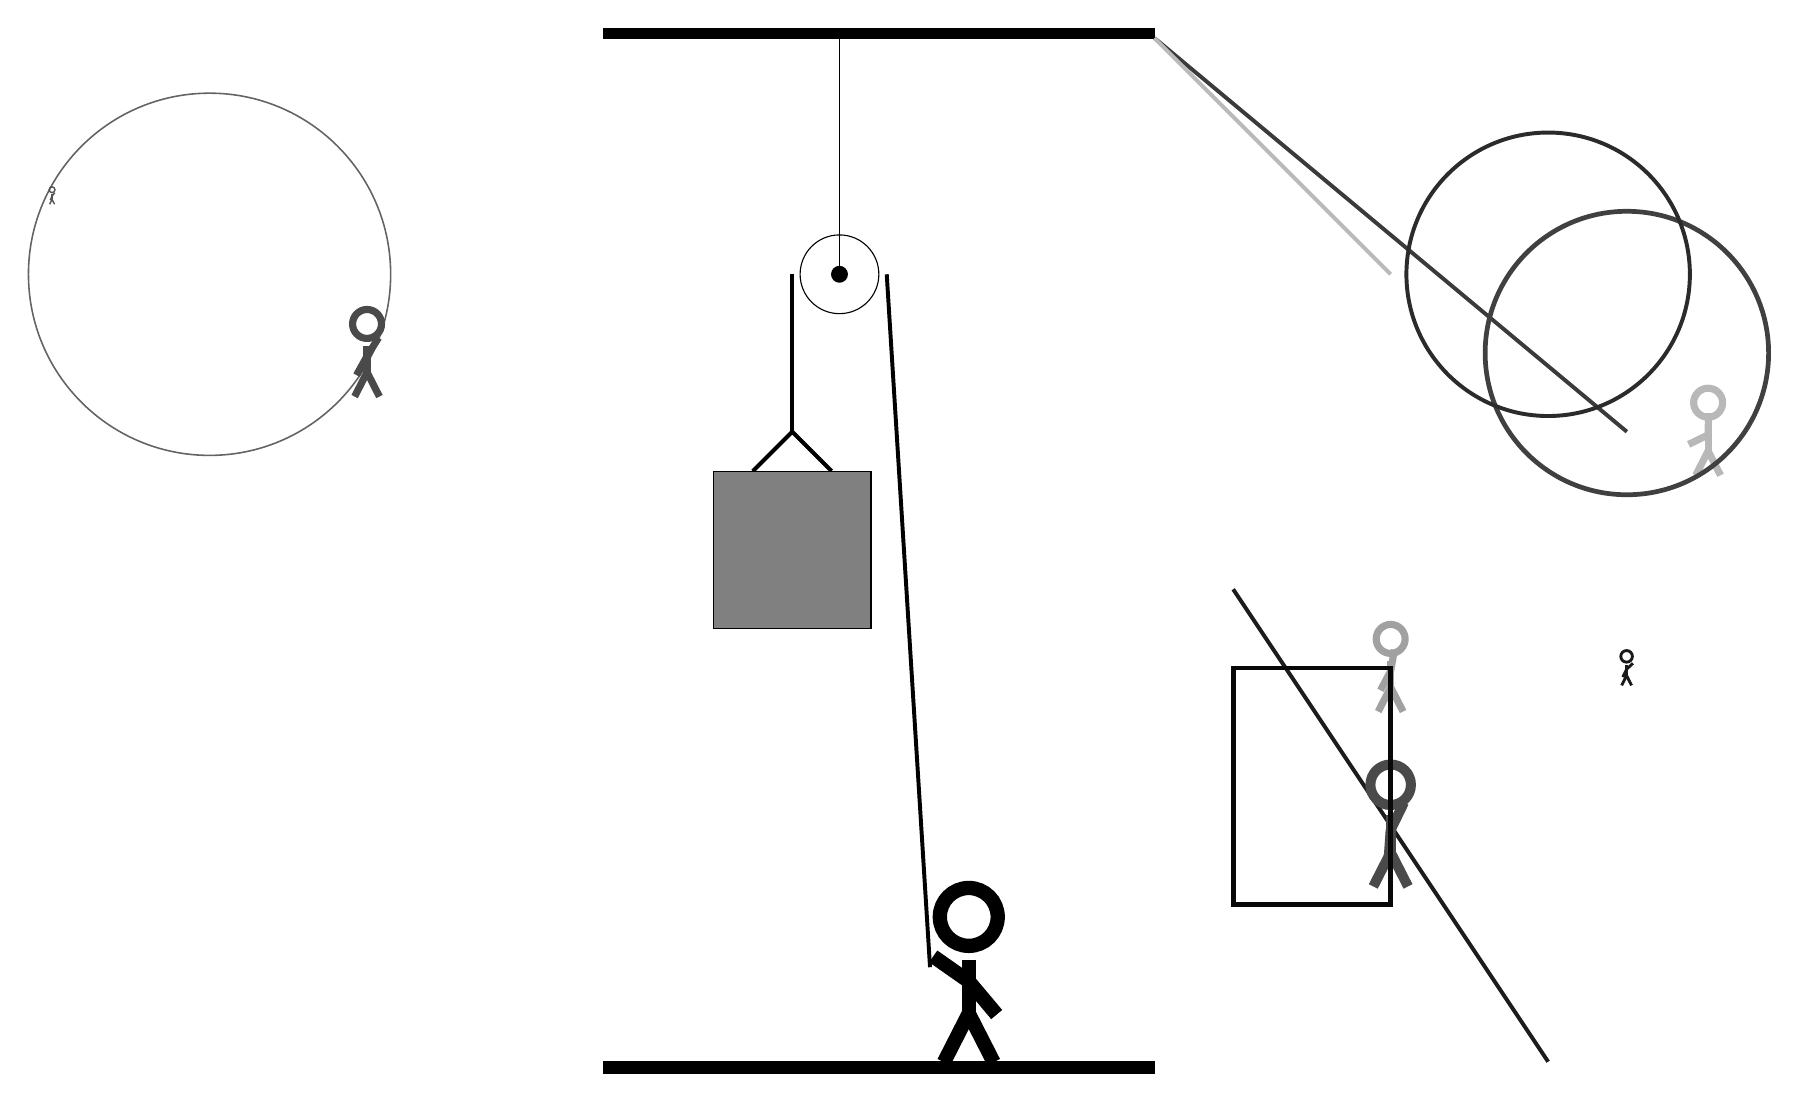
\begin{tikzpicture}
		%%%%% START %%%%%
		
		\draw[fill=black] (-2, 10) rectangle (5, 10.125);
		
		\draw (1, 7) circle (0.5);
		\draw[fill=black] (1, 7) circle (0.1);
		\draw (1, 10) -- (1, 7);
		
		\node[line width=0.3mm, color=black!28] at (12, 5) {\Strichmaxerl[5][26][89]};
		
		\draw [line width=0.2mm, color=black!61](-7, 7) circle (2.3);
		\node[line width=0.5mm, color=black!67] at (-9, 8) {\Strichmaxerl[1][65][52]};
		\draw [line width=0.6mm, color=black!73](-5, -3) circle (0.0);
		\draw[line width=0.5mm, color=black!89](10, -3) -- (6, 3);
		\draw[line width=0.5mm, color=black!77](5, 10) -- (11, 5);
		
		\node[line width=0.5mm, color=black!90] at (11, 2) {\Strichmaxerl[2][64][43]};
		\node[line width=0.6mm, color=black!71] at (8, 0) {\Strichmaxerl[7][86][64]};
		\node[line width=0.5mm, color=black!37] at (8, 2) {\Strichmaxerl[5][62][80]};
		\draw [line width=0.6mm, color=black!75](11, 6) circle (1.8);
		
		\draw [line width=0.5mm, color=black!83](10, 7) circle (1.8);
		\node[line width=0.3mm, color=black!71] at (-5, 6) {\Strichmaxerl[5][61][58]};
		\draw[line width=0.6mm, color=black!97] (6, -1) rectangle (8, 2);
		
		\draw[line width=0.5mm, color=black!27](5, 10) -- (8, 7);
		
		\draw[line width=0.5mm] (-0.1, 4.5) -- (0.4, 5.0) -- (0.9, 4.5);
		\draw[fill=black!50] (-0.6, 4.5) rectangle (1.4, 2.5);
		
		\draw[line width=0.5mm] (0.4, 7) -- (0.4, 5.0);
		\centerarc[line width=0.5mm](1, 7)(0:180:0.6);
		\draw[line width=0.5mm](1.6, 7) -- (2.15, -1.8);
		
		\node at (2.6, -1.9) {\Strichmaxerl[10][-35][-50]};
		
		\draw[fill=black] (-2, -3) rectangle (5, -3.15);
		
		%%%%% END %%%%%
	\end{tikzpicture}
\end{document}